%\documentclass[../../Orator]{subfiles}
\documentclass[class={myRUCProject}, crop=false]{standalone}
\IfStandalone{%
    \import{../../}{customCommands}
    \import{../../}{INP-00-glossary}
    }{}

\usepackage[subpreambles = true]{standalone}
\usepackage{myTikz}


\begin{document}


\begin{figure}[H]
    \centering
    \import{../../Pictures/Anakin}{Neuron.tex}
    \caption{A simplified representation of a \gls{gls:neuron}[al] cell, with labels for each of the important features. (1) the \gls{gls:soma} of the cell; (2) a \gls{gls:dendrite}; (3) the \gls{gls:axon}; (4) the \gls{gls:ax-hill}; (5) the \gls{gls:ax-terminal}.}\label{fig:Neuron}
\end{figure}

The human body is composed of a vast number of cells and complex interactions, how could anyone ever expect these meaty lumps we call `\textit{\glspl{gls:person}}' to coordinate properly without an equally complex system for the transfer of information? 
\Glspl{gls:neuron} are information highways made manifest in multi-cellular organisms. 
There exist many distinct types of \glspl{gls:neuron}, however, the underlying mechanisms of function stay the same.

\section{Cellular Structures}
\subsection{Organelles}
\begin{enumerate}

    \item \textbf{The Nucleus} is mainly found in the centre of the cell and is responsible for distinguishing between eukaryotic and prokaryotic cells - existing only in the first ones. It functions as the key factor in the cell's activities, it contains the cell's gentic information (DNA), and is where the DNA replication, transcription, and RNA processing all happen.
    \item \textbf{The Ribosomes}
    \item \textbf{The Golgi-Apparatus}
    \item \textbf{The Endoplasmic Reticulum}
    \item \textbf{The Lysosome}
    
\end{enumerate}

\subsection{Specialized Neuronal Structures}
There exist a number of important features that are foundational to the specialized functions found in the \glspl{gls:neuron};
\begin{enumerate}
    \item \glslink{gls:soma}{\textbf{The soma}} is the main body of the \gls{gls:neuron}. It is the space in which the nucleus resides, and by extension where protein production occurs. The nucleus can range from \qtyrange{3}{18}{\um} in diameter.
    \item \glslink{gls:dendrite}{\textbf{The dendrites}} of a \gls{gls:neuron} are extensions of the \gls{gls:membrane} with many branches. This overall shape and structure are metaphorically referred to as a `\textit{\gls{gls:denTree}}'\footnotemark. This is where the majority of \gls{gls:neuron} inputs are received, and carried by the `dendritic spine' down to the \gls{gls:soma}~\cite{}. \footnotetext{Greek root word `\textit{dendron}' meaning tree, translates to `tree tree'.}
    \item \glslink{gls:axon}{\textbf{The axon}} is a finer tendril that can extend tens, if not tens of thousands of times, the diameter of the \gls{gls:soma} in length. The \gls{gls:axon} primarily carries nerve signals away from the \gls{gls:soma} and carries some types of information back to it. Most \glspl{gls:neuron} have only one \gls{gls:axon}, but this \gls{gls:axon} will be able to undergo significant branching, enabling communication with many target cells. 
    \item \glslink{gls:ax-hill}{\textbf{The axon hill-lock}} is the part of the \gls{gls:axon} where it emerges from the \gls{gls:soma}. The region contains the greatest density of voltage-dependent sodium channels. This makes it the most easily excited part of the \gls{gls:neuron}~\cite{}. 
    \item \glslink{gls:ax-terminal}{\textbf{The axon terminal}} is found at the terminus of the \gls{gls:axon} and contains synapses. 
    \item \textbf{The myelin sheathe} is a lipid and protein comprised substance excreted from ??? cells that `sheathes' the \gls{gls:axon}, creating additional insulation for \gls{gls:capa}~\cite{}.
\end{enumerate}


\section{The Resting Membrane Potential} 
A fundamental component of cells is the \gls{gls:membrane}, composed of what is known as a `\gls{gls:bilipid}'\footnotemark. A \gls{gls:bilipid} creates a strong electrical insulation, 
which confers it the property of `\gls{gls:capa}'~\cite{}
%- the capability of an object to store electrical charge 
.  
In a \gls{gls:neuron}, the overall charge in the \gls{gls:incell} space is more negative relative to the \gls{gls:excell} space. This difference in charge at rest is known as the resting \gls{gls:mPote}, and it is essential for the \gls{gls:neuron}['s] ability to transmit electrical signals. 
\footnotetext{Latin root word `bi' meaning two, translates to `lipid two-layer'} 

By convention, membrane potential - or voltage \(\br{\unit{\V\membrane}}\) is the difference between the electric potential of the internal and external faces of the membrane \(\br{\unit{\V\membrane}=\unit{\V\incell}-\unit{\V\excell}}\). In the absence of ongoing electrical activity, this negative potential is termed the resting membrane potential \(\br{V_{rest}}\).  The usual resting \gls{gls:mPote} is found to be around \glslink{gls:volt}{\qty{-70}{millivolts\br{\milli\volt}}} in \glspl{gls:neuron}, however, it varies depending on the cell type and conditions~\cite{}. When the membrane potential is less negative than  \(V_{rest}\), the membrane is considered to be depolarized. In contrast, when the membrane potential is more negative than \(V_{rest}\), the membrane is said to be hyperpolarized \cite{Hammond2015ch3}. 

The \glspl{gls:ion} found to be involved in the \gls{gls:mPote} include \gls{Na}, \gls{K}, \gls{Cl}, and, to a limited degree, \gls{Ca}. 
In the \gls{gls:excell} space the concentrations of \gls{Na} and  \gls{Cl} are kept much higher than in the cytoplasm of the \gls{gls:incell} space, whereas \gls{K} is found in much higher concentrations in the cytoplasm compared to the \gls{gls:excell} space. During rest, their concentration \glspl{gls:grad} are actively regulated and maintained at constant values by `\glspl{gls:ionPump}', that chemically transport \glspl{gls:ion} across the \gls{gls:membrane}~\cite{}. However, the main contributors to the negative potential of the intracellular side of the memrane are the anions of the intracellular fluid, which are organic molecules such as negatively charged amino acids, proteins, nucleic acids, phosphates, etc., which have a large molecular weight and cannot cross the lipid membrane and thus do not participate directly in electrical signaling in neurons\cite{Hammond2015ch3}. 


An important structure embedded in the \gls{gls:bilipid} includes `\glspl{gls:ionChan}' which permit electrically charged \glspl{gls:ion} to diffuse across the \gls{gls:membrane} \gls{gls:grad}. \Glspl{gls:ionChan} are only permeable to a specific \gls{gls:ion}~\cite{}. Some \glspl{gls:ionChan} are voltage gated, meaning that they can be switched between open and closed states by altering the voltage across the \gls{gls:membrane}. 
Others are `\gls{gls:lig} gated', meaning that they can be switched between an open and a closed state by interacting with \glspl{gls:lig} that travel through the \gls{gls:excell} fluid. 

\vspace{1em}

\begin{figure}[H]
    \centering
    \import{../../Pictures/Anakin}{LipidCircuit.tex}
    \caption{The Hodgkin-Huxely circuit diagram overlaid with the relevant structures found in the \gls{gls:membrane}. \glssymbol{gls:excell} and \glssymbol{gls:incell} denote the \gls{gls:excell} space and the \gls{gls:incell} space respectively. \Gls{gls:capa} of the \gls{gls:membrane} \(\br{\cap\membrane}\) is given by the charge difference on either side of the \gls{gls:bilipid}. \Glspl{gls:ionChan} for \gls{Na} and \gls{K} are shown with the relevant variables, resistor type, and battery. Additional \glspl{gls:ionChan} and other leaked is represented as a lone resistor and battery outside of the \gls{gls:membrane} region. The \gls{K} \glspl{gls:ion} are shown in green, \gls{Na} are shown in red, and \gls{Cl} \glspl{gls:ion} in yellow; distributed in approximately relative concentrations on either side of the \gls{gls:membrane}. }\label{fig:MembraneCircut}
\end{figure}


\subsection{Ions Passively Diffuse Down Their Electrochemical Gradient}
The direction of the passive diffusion of \glspl{gls:ion} through an open channel depends on both the concentration \gls{gls:grad} of the \gls{gls:ion} and the \gls{gls:mPote}. The resultant of these two forces is called the electrochemical \gls{gls:grad}.

When  the \gls{gls:mPote} is null \(\br{\unit{\V\membrane}=\qty{0}{\mV}}\), there is no difference of \gls{gls:Pote} between the two faces of the \gls{gls:membrane}, so the concentration \gls{gls:grad} will be the only factor determining the direction of diffusion for specific \glspl{gls:ion} \cref{sfig:dirA}. Since the concentrations of \gls{Na}, \gls{Ca} and \gls{Cl}  in the \gls{gls:excell} fluid are higher than in the  \gls{gls:incell} medium, these \glspl{gls:ion} will diffuse passively towards the \gls{gls:incell} space (when \gls{Na}, \gls{Ca} or \gls{Cl} permeable channels are open) as a result of their concentration \gls{gls:grad}. In contrast, since \gls{K} is a lot more abundant in the intracellular \gls{gls:media}, it will move from the \gls{gls:incell} \gls{gls:media} to the \gls{gls:excell} one when \gls{K} permeable channels are open. 

If we suppose that there is the same concentration of each \gls{gls:ion} in the \gls{gls:excell} and \gls{gls:incell} \glspl{gls:media}, i.e there is no concentration \gls{gls:grad} for any \glspl{gls:ion}, \glspl{gls:ion} will diffuse according to \gls{gls:mPote} only: positive ions (cations) will move towards negative potential, negative ions (anions) will move towards postive potential. At a \gls{gls:mPote} \(\unit{\V\membrane}=\qty{-30}{\mV}\) \cref{sfig:dirB}, positively charged \glspl{gls:ion}, the \glspl{gls:cation} \gls{Na}, \gls{Ca} and \gls{K}, will move from the \gls{gls:excell} \gls{gls:media} to the \gls{gls:incell} one according to \gls{gls:mPote}. In contrast, \glspl{gls:anion} (\gls{Cl}) will move from the \gls{gls:incell} \gls{gls:media} to the \gls{gls:excell} one. 

%In physiological conditions, both the concentration \gls{gls:grad} and \gls{gls:mPote}  determine the direction and amplitude of \gls{gls:ion} diffusion through an open channel.
In physiological conditions, the concentration \gls{gls:grad} is maintained constant for each \gls{gls:ion}, so the direction and amplitude of diffusion mainly varies with \gls{gls:mPote}. When comparing \cref{sfig:dirA,sfig:dirB} it appears that the concentration \gls{gls:grad} and the \gls{gls:mPote} (at  \(\qty{-30}{\mV}\)) drive \gls{Na} and \gls{Ca} \glspl{gls:ion} in the same direction, toward the \gls{gls:incell} \gls{gls:media}, whereas the direction that \gls{K} and \gls{Cl} ions are driven is reversed . The resultant of these two forces, concentration and \gls{gls:Pote} \glspl{gls:grad}, is the electrochemical \gls{gls:grad}. To know how to express the electrochemical \gls{gls:grad}, the \gls{gls:ePote} must first be explained.
 
\begin{figure}[H]
    \begin{subfigure}[t]{0.45\textwidth}
        \centering
        \caption{}\label{sfig:dirA}
        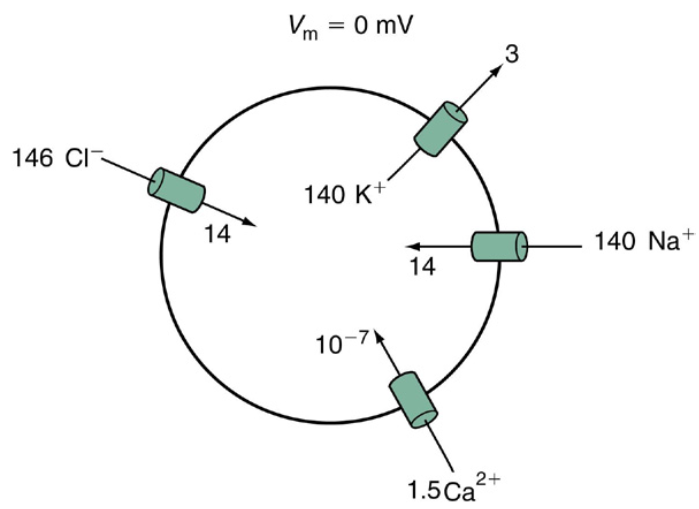
\includegraphics[height=6cm]{Pictures/Anakin/c.grad.png}
    \end{subfigure}
    \hfill
    \begin{subfigure}[t]{0.45\textwidth}
        \centering
        \caption{}\label{sfig:dirB}
        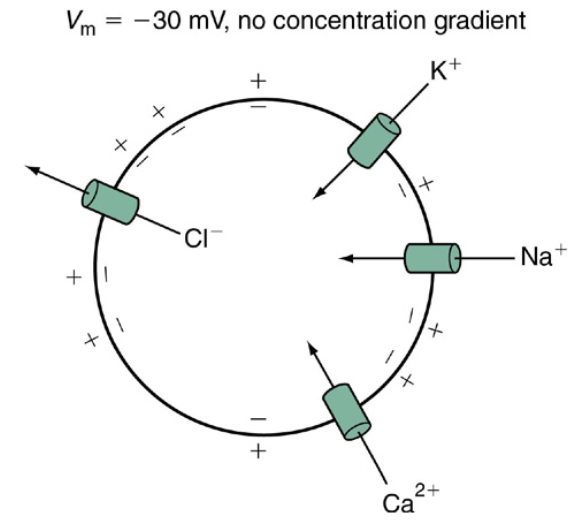
\includegraphics[height=6cm]{Pictures/Anakin/el.grad.png}
    \end{subfigure}
      \caption{Passive diffusion of \glspl{gls:ion}. Passive diffusion of \glspl{gls:ion}  according \labelcref{sfig:dirA} their concentration \gls{gls:grad} only, or \labelcref{sfig:dirB} to \gls{gls:membrane} \gls{gls:Pote} (electrical \gls{gls:grad}) only \(\br{\unit{\V\membrane} = \qty{-30}{\mV}}\). From \cite{Hammond2015ch3}}\label{fig:direction} 
\end{figure}


\subsection{Equilibrium Potential of a Given Ion}
\begingroup
\allowdisplaybreaks
All systems yearn for their \gls{gls:equil}, the fabled \textit{steady state}. This divine relation of the components in a system, one achieved, the system no longer needs to evolve, it has been perfected by entropy. 
The value of the \gls{gls:mPote} is constantly fluctuating depending on the relative distribution of charged particles that cross the \gls{gls:membrane}. 
When the direction of the \gls{gls:grad} is perfectly balanced at net zero, it is referred to as the `\gls{gls:ePote}' of the given \gls{gls:ion} \br{\equilibria\ion}, alternatively, as the `\gls{gls:rPote}' of the \gls{gls:ion} \(\equilibria\reverse\). 
%The \gls{gls:ePote} for a particular \gls{gls:ion} is the value of \(\unit{\V\membrane}\) for which the net \gls{gls:flux} of this \gls{gls:ion}\(\br{f_\bfm{net}}\) through an open channel is null: when \(\unit{\V\membrane} = \equilibria\ion\), \(f_\bfm{net} = \qty{0}{\mole\per\second}\).
The \(\equilibria\ion\) of the given \glspl{gls:ion} can be calculated using the \textit{Nernst} equation:
\begin{subequations}\label{eq:nernst}
\begin{equation}
    \equilibria\ion = \br{\frac{\clm{R}\, \cdot \,\clm{T}}{z\, \cdot \, \clm{F}}} \, \ln \br{\frac{\ionconc\excell }{ \ionconc\incell} } \tag{\ref*{eq:nernst}} 
\end{equation}

Where \(\clm{R}\) is the ideal gas constant \br{\qty{8.314}{\cubic\meter\pascal\per\kelvin\per\mol}}; \(\clm{T}\) is the temperature in \gls{gls:kelvin} \(\br{ x\,\unit{\glssymbol{gls:celsius}} \cong {273.15} + x\,\unit{\kelvin}}\); \(\clm{F}\) is the Faraday constant \br{\qty{96500}{\coulomb\per\mole}}; \(z\) is the valence of the \gls{gls:ion}; and \(\ionconc\) is the concentration of the given \gls{gls:ion} in the \gls{gls:excell} \( \br{ \clm{E} } \) or \gls{gls:incell} \( \br{\clm{I}}\) \gls{gls:media}. 
As most of these terms are constants, it is simple to reduce the equation down in dimensional complexity:
\begin{align} 
    \equilibria\ion &= \br{\frac{ \qty{8.314}{\cubic\meter\pascal\per\mol\per\kelvin} \, \cdot \, \clm{T}}{ z\, \cdot \, \qty{96500}{\coulomb\per\mole} }} \,\ln \br{ \frac{ {\ionconc\excell} }{ {\ionconc\incell}} } \\
    %\equilibria\ion &= \br{\frac{ {8.314} \cdot \(t\) \cdot \unit{\cubic\meter\pascal}  \,\cancel{\unit{\per\mol}}\,\cancel{\unit{\per\kelvin\kelvin}}  }{ z\, \cdot \, \qty{96500}{\coulomb} \,\cancel{\unit{\per\mol}}}} \,\ln \br{ \frac{ {\ionconc\excell} }{ {\ionconc\incell}} } \\
    %
    %\equilibria\ion &= \br{\frac{ {8.314} \, \cdot \,  \(t\) \, \unit{\cubic\meter\pascal} }{ z\, \cdot \, \qty{96500}{\coulomb}} } \,\ln \br{ \frac{ {\ionconc\excell} }{ {\ionconc\incell}} } \\
    %
    \intertext{dividing and rearranging the terms:}
    \equilibria\ion &= \br{\frac{ \clm{T}\unit{\per\K} \, \unit{\cubic\meter\pascal} }{ z\, \cdot \, \qty{11612.515042118}{\coulomb} } } \cdot \,\ln \br{ \frac{ {\ionconc\excell} }{ {\ionconc\incell}} } \\
    %
    \intertext{converting the unit of pressure, pascal \br{\unit{\pascal}} to the base units representing mass over an area over time \br{\unit{\kilo\gram\per\meter\per\square\second}}, as well converting the unit for charge, a \gls{gls:coulomb} \br{\unit{\coulomb}}, to the base units denoting the quantity of current in a second, \br{\unit{\ampere\second}}, gives the substitution:}
    \equilibria\ion &= \br{\frac{ \clm{T}\unit{\per\K} \, \unit{\cubic\meter\kilo\gram\per\meter\per\square\second} }{ z\, \cdot \, \qty{11612.515042118}{\ampere\second} } } \cdot \,\ln \br{ \frac{ {\ionconc\excell} }{ {\ionconc\incell}} } \\
    \intertext{at this point we're only left with base SI units, so we need to be a little silly, the unit of magnetic \gls{gls:flux} is defined \(\unit{\weber} = \unit{\kilo\gram\square\meter\per\square\second\per\ampere}\), implying through substitution \(\unit{\kilo\gram\square\meter\per\cubic\second\per\ampere} = \unit{\weber\per\second} \):}
    \equilibria\ion &= \frac{ \clm{T}\unit{\per\K}  }{ z\, \cdot \, \num{11612.515042118}} \cdot \br{\unit{\weber\per\second}} \cdot \,\ln \br{ \frac{ {\ionconc\excell} }{ {\ionconc\incell}} } \\
    %
    \intertext{a unit describing the rate of change of magnetic charge per second, which is equivalent to a Volt, \(\unit{\weber\per\second}  = \unit{\volt} = \unit{\kilo\gram\square\meter\per\cubic\second\per\ampere} \), the combination of units found through deconstruction is the literal base unit definition of a volt:}
    \equilibria\ion &= \frac{ \clm{T}\unit{\per\K} }{ z\, \cdot \, \num{11612.515042118}} \cdot \unit{\volt} \cdot \ln \br{ \frac{ {\ionconc\excell} }{ {\ionconc\incell}} }\label{eq:derivedNerst}
    %\equilibria\ion &= \cfrac{ \(t\) \cdot \,\ln \br{ \cfrac{\ionconc\excell }{ \ionconc\incell} }  }{ z\, \cdot \, \num{11612.515042118}}  \cdot \unit{\volt} \cdot  \qty{1000}{\milli\volt\per\volt} \\
    %\equilibria\ion &= \cfrac{ \(t\) \cdot \,\ln \br{ \cfrac{\ionconc\excell }{ \ionconc\incell} } }{ z\, \cdot \, 1 \, 160}  \ \unit{\milli\volt}
\end{align}
%{Volume Concentration \per\kelvin\per\mol}
%{\kilo\gram\metre^2\second^{-2}\kelvin\per\mol}
\end{subequations}

\begin{subequations}\label{eq:mVions}
With minor adjustments to \cref{eq:derivedNerst}, the now derived form of \cref{eq:nernst}, one is able to get
\begin{equation}
    \equilibria\ion = \cfrac{\clm{T}\unit{\per\K}}{ z } \, \cdot \, \ln \br{ \frac{ {\ionconc\excell} }{ {\ionconc\incell}} } \cdot \num{11.612515042}^{-1}  \ \unit{\milli\volt} \tag{\ref*{eq:mVions}}
\end{equation}

Plugging the relative concentrations, measured in millimols \br{\unit{\milli\mol}}, of each \gls{gls:ion} into \cref{eq:mVions}, as well as choosing an arbitrary temperature, such as room temperature \(\approx\) \qty{20}{\degreeCelsius} \(\br{\br{\num{20} + \num{273.15}}\unit{\glssymbol{gls:kelvin}}}\),
the \gls{gls:ePote} of each \gls{gls:ion}follows as:
\begin{minipage}{.48\textwidth}
    \begin{align}
        {\equilibria\sodium} &= \num{293.15}\  \ln \br{ \frac{140}{14} }\cdot \num{11.612515042}^{-1} =  \qty{58.127185848}{\mV} \\
        {\equilibria\potassium}    &= \num{293.15}\  \ln \br{ \frac{3}{140} }\cdot \num{11.612515042}^{-1}  =  \qty{-97.014667339}{\mV} 
    \end{align}
\end{minipage}
~
\begin{minipage}{.48\textwidth}
    \begin{align}
        {\equilibria\calcium}   &= \frac{293.15}{2}\  \ln \br{ \frac{1.5}{10^{-4}} }\cdot \num{11.612515042}^{-1} =  \qty{121.372216367}{\mV} \\
        {\equilibria\chlorine}   &= \num{-293.15}\ \ln \br{ \frac{146}{14} }\cdot \num{11.612515042}^{-1} =  \qty{-59.186543354}{\mV} 
    \end{align}
\end{minipage}

\end{subequations}

These equations can be interpreted such that when
\gls{K} channels open in the \gls{gls:membrane}, the efflux of \gls{K} \glspl{gls:ion} will hyper-polarize the \gls{gls:membrane} until \(\unit{\V\membrane} = \equilibria\potassium \approx \qty{-97}{\mV}\), at which point the net \gls{gls:flux} of \gls{K} is null being that \gls{K} \glspl{gls:ion} have exactly the same \gls{gls:Pote} to move towards the \gls{gls:excell} space as the \gls{gls:incell} space. 
The efflux of \gls{K} will be exactly compensated by the influx of \gls{K} and the \gls{gls:mPote} will stabilize at \equilibria\potassium for as long as the \gls{K} channels stay open. 
Assuming only \gls{Na} channels are open, the \gls{gls:mPote} will move toward \(\unit{\V\membrane} = \qty{58}{\mV}\), the \gls{gls:Pote} at which the net \gls{gls:flux} of \gls{Na} is null. 
Similarly, when \(\unit{\V\membrane} = \equilibria\chlorine \approx \qty{-59}{\mV}\),  
%\gls{Cl} \glspl{gls:ion} have the  tendency to move down their concentration \gls{gls:grad} than to move in the reverse direction according to \gls{gls:mPote}, 
the net \gls{gls:flux} of \gls{Cl} is null. 
By extension, should \(\unit{\V\membrane} \neq \equilibria\potassium\), the net \gls{gls:flux} of  \gls{K} will no longer be null. 
This holds true for all \glspl{gls:ion}: when \(\unit{\V\membrane} \neq \equilibria\ion\) there is a net \gls{gls:flux} of the \gls{gls:ion}~\cite{}. The difference \(\br{\unit{\V\membrane} - \equilibria\ion}\) is called the electrochemical \gls{gls:grad}. It is the force that makes the \glspl{gls:ion} move through an open channel.

\endgroup

\subsection{Ionic currents}
The passive diffusion of \glspl{gls:ion} through an open channel is a movement of charge through a resistance (resistance here is a measure of the difficulty of \glspl{gls:ion} moving through the channel pore). Movement of charges through a resistance is a current. Through a single channel the current is called `single-channel current' or `unitary current', \(\uncur\ion\). The amplitude of  \(\uncur\ion\) is expressed in amperes \(\br{\unit{\ampere}}\) which are coulombs per seconds \(\br{\unit{\coulomb\per\second}}\). 

In general, currents are expressed following ohm's law: U=RI, where I is the current through a resistance R and U is the difference of \gls{gls:Pote} between the two ends of the resistance. For currents carried by \glspl{gls:ion} (and not by electrons as in copper wires), I is called  \(\cur\ion\), the current that passes through the resistance of the channel pore which has a resistance R \(\br{\res\ion}\). But what is U in biological systems? U is the force that makes \glspl{gls:ion} move in a particular direction; it is the electrochemical \gls{gls:grad} for the considered \gls{gls:ion} and is also called the driving force: \(U=(\unit{\V\membrane} - \equilibria\ion)\). According to ohm's law, the current \(\cur\ion\) through a single channel is derived from 
\begin{equation}
    \unit{\V\membrane} - \equilibria\ion = r_{ion} \cdot \cur\ion
\end{equation}
So:
\begin{equation}
    \cur\ion= \frac{1}{r_{ion}\br{\unit{\V\membrane} - \equilibria\ion}} = \uncon\ion(\unit{\V\membrane} - \equilibria\ion)
\end{equation}
\(\uncon\ion\) is the reciprocal of resistance; it is called the \textit{\gls{gls:contan}} of the channel, or unitary \gls{gls:contan}. It is a measure of the ease of flow of \glspl{gls:ion} (flow of current) through the channel pore. Whereas resistance is expressed in ohms \(\br{\unit{\ohm}}\), \gls{gls:contan} is expressed in siemens \(\br{\unit{\siemens}}\). By convention \(\cur\ion\) is negative when it represents an inward \gls{gls:flux} of positive charges (\glspl{gls:cation}) and \(\cur\ion\) is positive when it represents an outward \gls{gls:flux} of positive charges. It is generally of the order of pico-amperes \(\br{\qty{1}{\pico\ampere}=\qty{e-12}{\ampere}}\). At physiological concentrations, \(\uncon\ion\) varies between \(\qtyrange{10}{150}{\pico\siemens}\) dependent on channel type~\cite{}.

In physiological conditions, however,  several channels of the same type are open at the same time in the \gls{gls:neuron}[al] \gls{gls:membrane}. Suppose that only one type of channel is open in the \gls{gls:membrane}, for example \gls{Na} channels, the total current \(\unit{\cur\sodium}\) crossing the \gls{gls:membrane} at time \(t\) is the sum of the unitary currents \(\unit{\uncur\sodium}\) at time \(t\):
\begin{equation}
    \unit{\cur\sodium} = N \, p_o \, \unit{\uncur\sodium}
\end{equation}
where \(N\) is the \emph{number} of \gls{Na} channels present in the \gls{gls:membrane}; \(p_o\) is the \emph{probability} of \gls{Na} channels being open at time \(t\)
%(\(N\,p_o\) is therefore the number of open \gls{Na}channels in the \gls{gls:membrane} at time \(t\))
; and \(\unit{\uncur\sodium}\) is the unitary \gls{Na} current.  \newline
More generally:
\begin{equation}
    \cur\ion= N \, p_o \, \uncur\ion
\end{equation}
By analogy, the total \gls{gls:contan} of the \gls{gls:membrane} for a particular \gls{gls:ion} is: 
\begin{equation}
    \unit{\con\ion} = N \, p_o \, \uncon\ion
\end{equation}
and from \(\cur\ion= \uncon\ion \, \br{\unit{\V\membrane} - \equilibria\ion}\) above: 
\begin{equation}\label{eq:ionCurrent}
    \cur\ion= \unit{\con\ion} \, \br{\unit{\V\membrane} - \equilibria\ion}
\end{equation}
\(\uncur\ion\) and \(\cur\ion\) can be measured experimentally. The former is the current measured from a patch of \gls{gls:membrane} where only one channel of a particular type is present. \(\cur\ion\) is the current measured from a whole cell \gls{gls:membrane} where \(N\) channels of the same type are present. 
 
\section{Action Potential}

Functionally all eukaryotic \glspl{gls:membrane} maintain a difference in voltage between the \gls{gls:excell} and \gls{gls:incell} space, this difference is called the `\gls{gls:mPote}'. The expected \gls{gls:mPote} in human cells is \glslink{gls:volt}{\qty{-70}{\milli\volt}}~\cite{}.
\gls{ap} is the measure of the \gls{gls:Pote} that causes action.

An \gls{ap} occurs when the \gls{gls:Pote} of an excitable cell's \gls{gls:membrane} rapidly rises and falls. This \gls{gls:depol} then causes adjacent regions to similarly `depolarize', creating a chain reaction in the form of a `wavelet'.
The voltage fluctuations take the form of a rapid upward spike followed by a rapid fall.

``All-or-none'' principle

\begin{figure}[H]
    \centering
    \import{../../Pictures/Anakin}{Channels.tex}
    \caption{ $\langle \text{temp} \rangle$ }\label{fig:Channels}
\end{figure}

\begin{comment}
    Each excitable patch of \gls{gls:membrane} has two important levels of \gls{gls:mPote}: the resting potential, which is the value the \gls{gls:mPote} maintains as long as nothing perturbs the cell, and a higher value called the \gls{gls:tPote}. At the axon hillock of a typical \gls{gls:neuron}, the resting \gls{gls:Pote} is around –70 millivolts (mV) and the threshold \gls{gls:Pote} is around –55 mV. Synaptic inputs to a \gls{gls:neuron} cause the \gls{gls:membrane} to depolarize or hyperpolarize; that is, they cause the \gls{gls:mPote} to rise or fall. \glspl{ap} are triggered when enough \gls{gls:depol} accumulates to bring the \gls{gls:mPote} up to threshold. When an \gls{ap} is triggered, the \gls{gls:mPote} abruptly shoots upward and then equally abruptly shoots back downward, often ending below the resting level, where it remains for some period of time. The shape of the \gls{ap} is stereotyped; this means that the rise and fall usually have approximately the same amplitude and time course for all \glspl{ap} in a given cell. (Exceptions are discussed later in the article). In most \glspl{gls:neuron}, the entire process takes place in about a thousandth of a second. Many types of \glspl{gls:neuron} emit \glspl{ap} constantly at rates of up to 10–100 per second. However, some types are much quieter, and may go for minutes or longer without emitting any \glspl{ap}.

    \glspl{ap} result from the presence in a cell's \gls{gls:membrane} of special types of voltage-gated \glspl{gls:ionChan}.[6] A voltage-gated \gls{gls:ion}channel is a transmembrane protein that has three key properties:

    It is capable of assuming more than one conformation.
    At least one of the conformations creates a channel through the \gls{gls:membrane} that is permeable to specific types of \glspl{gls:ion}.
    The transition between conformations is influenced by the \gls{gls:mPote}.
    Thus, a voltage-gated \gls{gls:ion}channel tends to be open for some values of the \gls{gls:mPote}, and closed for others. In most cases, however, the relationship between \gls{gls:mPote} and channel state is probabilistic and involves a time delay. \Glspl{gls:ionChan} switch between conformations at unpredictable times: The \gls{gls:mPote} determines the rate of transitions and the probability per unit time of each type of transition.
\end{comment}
%original text
The \gls{ap} is a sudden and rapid \gls{gls:depol} of the \gls{gls:membrane} as a result of positive inward current \gls{gls:flux} through the \gls{gls:axon} segment. In \gls{gls:neuron}[al] \glspl{gls:soma} and \glspl{gls:axon}, these currents are most commonly propogated by \gls{Na} \glspl{gls:cation}\footnote{A positively charged \gls{gls:ion}, no relation to felines}.

The \gls{gls:ion}[ic] basis for \gls{gls:neuron}[al] excitation was first described in the giant squid axon by Hodgkin \& Huxley \br{1952} using the voltage clamp technique. They observed a key phenomenon, that the \gls{ap} is underlied by two separate voltage-dependent currents: an early transient inward \gls{Na} current which depolarizes the \gls{gls:membrane}, and a delayed outward \gls{K} current largely responsible for \gls{gls:repol}. The resulting voltage waveform takes the shape of a rapid upward spike followed by a rapid inactivation that eventually slightly hyperpolarizes the \gls{gls:membrane} before returning to resting \gls{gls:mPote} \Cref{fig:AP}.

Up to a threshold level of \gls{gls:membrane} \gls{gls:depol} (called the \gls{gls:tPote}), only passive ohmic response can be recorded, when the \gls{gls:membrane} is depolarized just above the threshold, an \gls{ap} is evoked. 
Increasing the intensity of the stimulating current pulse does not increase the amplitude of the \gls{ap},  the \gls{ap} is all or none. 
\begin{figure}[H]
    \centering
    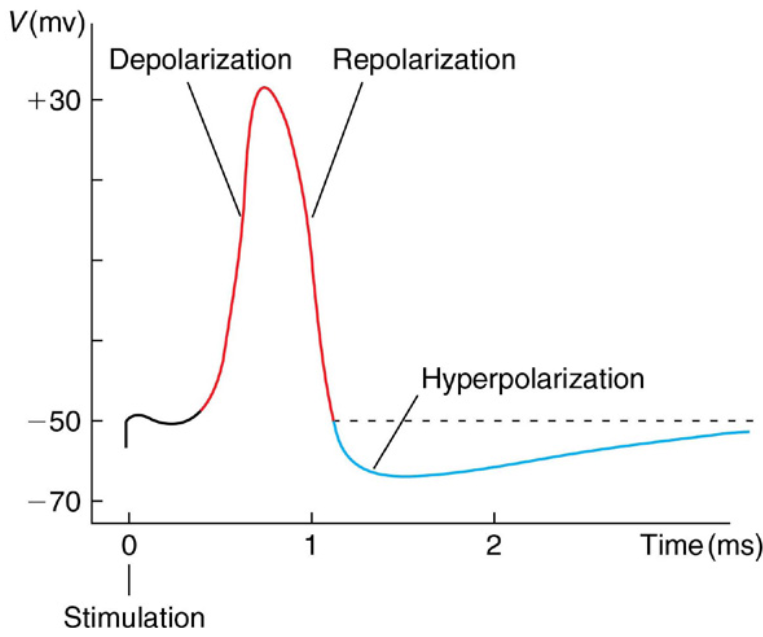
\includegraphics[width=0.5\linewidth]{Pictures//Anakin/AP.png}
    \caption{The \gls{ap} spike, indicating the different phases.}
    \label{fig:AP}
\end{figure}

\subsubsection{The depolarization phase of sodium-dependent action potential results from the transient entry of sodium ions through voltage gated sodium channels.}
%\subsubsection{The \gls{gls:depol} phase of \gls{Na}-dependent \gls{ap} results from the transient entry of \gls{Na} \glspl{gls:ion} through voltage gated \gls{Na} channels.}
The threshold  for initiation of \gls{Na}-dependent  action  \gls{gls:Pote} is due to the fact that voltage-gated \gls{Na} channels open only  in  response  to  a  \gls{gls:depol}  positive  of \qtyrange{-50}{-40}{\mV}, hence the name `voltage-gated'. 

In response to a \gls{gls:depol} to the \gls{gls:tPote}, the closed \gls{Na} channels of the axon initial segment begin to open. The \gls{gls:flux} of \gls{Na} \glspl{gls:ion} through the few open \gls{Na} channels depolarizes the \gls{gls:membrane} more and thus triggers the opening of other \gls{Na} channels. In consequence, the \gls{gls:flux} of \gls{Na} \glspl{gls:ion} increases, depolarizes the \gls{gls:membrane} more and opens other \gls{Na} channels until all the \gls{Na} channels of the segment of \gls{gls:membrane} are opened, which is when the \gls{gls:depol} phase is at its peak. \gls{Na} channels are opened by \gls{gls:depol} and once opened, they contribute to the \gls{gls:membrane} \gls{gls:depol} and therefore to their activation: it is a self-maintained process, which is why the  \gls{Na}-dependent  action  \gls{gls:Pote}  is  all  or  none. Once initiated, the \gls{ap} propagate along the axon without decaying, with a speed varying from \qtyrange{1}{100}{\m\per\s} depending on the type of \gls{gls:axon}.  It  propagates  without  attenuation  since  the  density of voltage-gated \gls{Na} channels is constant along the  axon as well as due to the presence of the insul ating myelin sheathe.  Once the channels inactivate, they may not reopen, which ensures that \gls{ap} only propagates  unidirectionally forward. 
%originaltextend
The time during which the \gls{Na} channel stays open varies around an average value, \(\tau_O\), called the mean open time. The functional significance of this value is the following: during a time equal to \(\tau_O\) the channel has a high probability of staying open. 

The \unit[per-mode = symbol]{\cur\sodium\per\V} relation is obtained by plotting the amplitude of the unitary current \(\br{\cur\sodium}\) versus \gls{gls:mPote} \(\br{\unit{\V\membrane}}\). It is linear between \qtyrange{-50}{0}{\mV}. For \glspl{gls:mPote} more hyperpolarized than \qty{-50}{\mV}, there are no values of \unit{\cur\sodium} since the channel rarely opens or does not open at all. Quantitative data for potentials more depolarized than \qty{0}{\mV} are not available.

When the activity of a single \gls{Na} channel is  recorded at different test potentials, it was observed that the amplitude of the inward unitary current \(\br{\cur\sodium}\) diminishes as the \gls{gls:membrane} is further and further depolarized. The critical point of the current/voltage relation is the \gls{gls:mPote} for which the current is zero; i.e. the reversal \gls{gls:Pote} of the current (\equilibria\reverse). If only \gls{Na} \glspl{gls:ion} flow through the \gls{Na} channel, the reversal \gls{gls:Pote} is equal to \equilibria\sodium. From \qty{-50}{\mV} to \equilibria\reverse, \unit{\cur\sodium} is inward and its amplitude decreases. This results from the decrease of the \gls{Na} driving force \(\br{\unit{\V\membrane}-\equilibria\sodium}\) as the \gls{gls:membrane} approaches the reversal \gls{gls:Pote} for \gls{Na} \glspl{gls:ion}. For \glspl{gls:mPote} more depolarized than \equilibria\reverse, \unit{\cur\sodium} is now outward. Above \equilibria\reverse, the amplitude of the outward \gls{Na} current progressively increases as the driving force for the exit of \gls{Na} \glspl{gls:ion} increases. 

The linear \unit[per-mode = symbol]{\cur\sodium\per\V}relation is described by the equation \(\unit{\cur\sodium} = \unit{\con\sodium} \br{\unit{\V\membrane}-\equilibria\sodium}\), where \unit{\V\membrane} is the test potential, \equilibria\sodium is the reversal \gls{gls:Pote} of the \gls{Na} current, and \unit{\con\sodium} is the \gls{gls:contan} of a single \gls{Na} channel (unitary \gls{gls:contan}). The value of \unit{\con\sodium} is given by the slope of the linear \unit[per-mode = symbol]{\cur\sodium\per\V} curve. It has a constant value at any given \gls{gls:mPote}. This value varies between \qtyrange{5}{18}{\pico\second} depending on the preparation.

\begin{figure}[H]
    \centering
    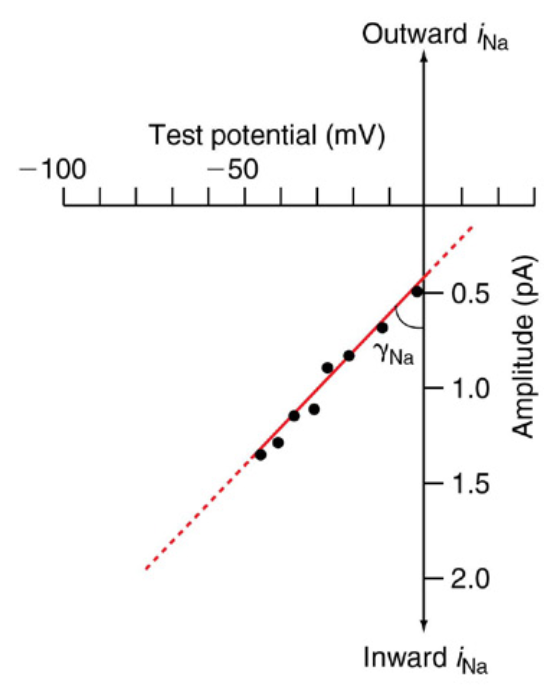
\includegraphics[width=0.5\linewidth]{Pictures//Anakin/iNa-VNa.png}
    \caption{The single-channel current/voltage \br{\unit[per-mode = symbol]{\cur\sodium\per\volt}} relation is linear. }
    \label{fig:NaVNa}
\end{figure}
The open probability of the voltage-gated \gls{Na} channel is voltage and time dependent. During cell recordings of \gls{Na} channels, it was observed that when the \gls{gls:mPote} is depolarized, the probability of the \gls{Na} channel being in the open state increases with \gls{gls:depol} to a maximal level. The higher is the depolarizing step, the higher is the probability of the \gls{Na} channel opening. It also varies with time during the depolarizing step: openings occur more frequently at the beginning of the step. It was observed  that after \qtyrange{4}{6}{\ms} the probability of the \gls{Na} channel being in the open state is very low, even with large depolarizing steps: the \gls{Na} channel in-activates in \qtyrange{4}{6}{\ms}.  The probability of the \gls{Na} channel being in the open state at time \(t=\qty{2}{\ms}\), for example, increases with the amplitude of the depolarizing step. To generalize, at \qty{-30}{\mV} the open probability is maximum, and the channels inactivate in \qty{4}{\ms}. 

\(\unit{\cur\sodium}\) is the macroscopic current, or the sum of all unitary currents, \unit{\cur\sodium} flowing through all the open \gls{Na} channels of the recorded \gls{gls:membrane}. In Figure 7b, an average of \(\num{300}\) unitary \gls{Na} currents elicited by a \(\qty{40}{\mV}\) depolarizing pulse is shown. For a given potential, the `averaged' inward \gls{Na} current has a fast rising phase and presents a peak at the time \(t=\qty{1.5}{\ms}\). The peak corresponds to the time when most of the \gls{Na} channels are opened at each trial. Then the averaged current decays with time because the \gls{Na} channel has a low probability of being in the open state later in the step (owing to the inactivation of the \gls{Na} channel). At each trial, the \gls{Na} channel does not inactivate exactly at the same time, which explains the progressive decay of the averaged macroscopic \gls{Na} current. A similar averaged \gls{Na} current is shown in Figure 4.8b. %The averaged current does not have a rectangular shape because the \gls{Na} channel does not open with the same delay and does not inactivate at the same time at each trial. 

\begin{figure}[H]
    \centering
    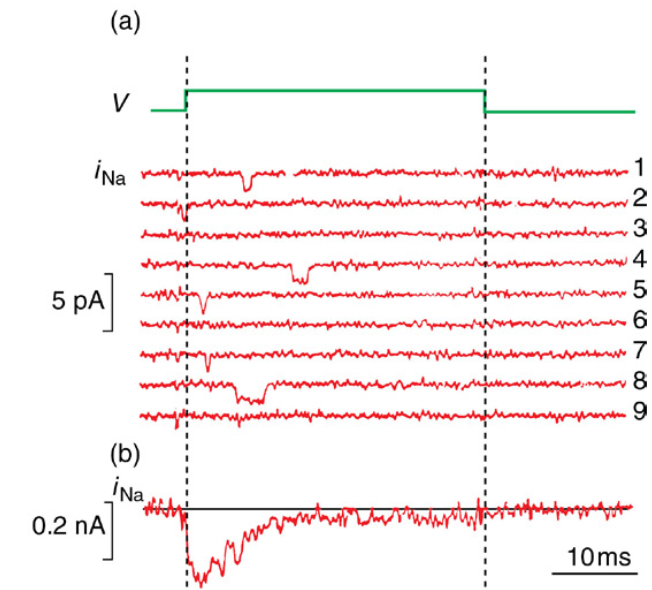
\includegraphics[width=0.5\linewidth]{Pictures//Anakin/iNa.png}
    \caption{Single \gls{Na} channel openings in response to adepolarizing step. (a) Nine successive recordings of single channel openings (iNa) in response to a\qty{ 40}{\mV} depolarizing pulse (V trace in green) applied at 1s intervals from resting \gls{gls:mPote}. (b) Averaged inward \gls{Na} current from 300 elementary \gls{Na} currents as in (a).  }
    \label{fig:enter-label}
\end{figure}

The greater the quantity of \gls{Na} channels open from the depolarizing step, the smoother the total \gls{Na} current. The value of \(\unit{\cur\sodium}\) at each time \(t\) at a given \gls{gls:Pote} is: 
\begin{equation}
    \unit{\cur\sodium}=N p_{(t)} \unit{\uncur\sodium}
\end{equation}
where \(N\) is the number of \gls{Na} channels in the recorded \gls{gls:membrane} and p(t) is the open probability at time \(t\) of the \gls{Na} channel; it depends on the \gls{gls:mPote} and on the channel opening and inactivating rate constants. \unit{\cur\sodium} is the unitary \gls{Na} current and Np(t) is the number of \gls{Na} channels open at time \(t\). 

Subsequently, the relation of the macroscopic \gls{Na} current \(\unit{\cur\sodium}\) and voltage \(\unit{\V}\) is not linear, but rather has a clear bell shape, with a peak at around \qty{-40}{\mV}. 
\begin{figure}[H]
    \centering
    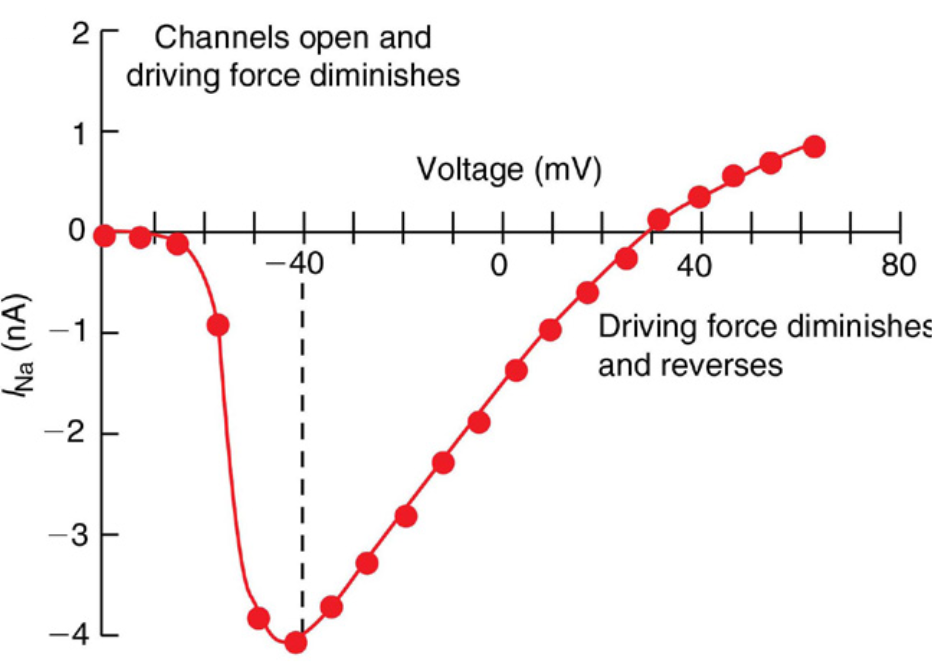
\includegraphics[width=0.5\linewidth]{Pictures//Anakin/I-V.bell.png}
    \caption{The INa-V relation has a bell shape. (From Chiu Sy, ritchie JM, bogart rb, Stagg d (1979) A quantitative description of \gls{gls:membrane} currents from a rabbit myelinated nerve. J. Physiol.292, 149–166)}
    \label{fig:enter-label}
\end{figure}
 
For small steps, the peak current amplitude is small \(\br{\qty{0.2}{\nano\ampere}}\) and has a slow time to peak \(\br{\qty{1}{\milli\second}}\). At these potentials, the \gls{Na} driving force is strong but the \gls{Na} channels have a low probability of opening. Therefore, INa is small since it represents the current through a small number of open \gls{Na} channels. 

As the depolarizing steps increase in amplitude (to -42/\qty{-35}{\mV}), the amplitude of INa increases to a maximum (\qty{-3}{\nA}) and the time to peak decreases to a minimum (\qty{0.2}{\ms}). Larger \glspl{gls:depol} increase the probability of the \gls{Na} channel being in the open state and shorten the delay of opening. Therefore, though the amplitude of iNa decreases by \qtyrange{-63}{-35}{\mV}, the amplitude of INa increases owing to the large increase of open \gls{Na}channels. 

After this peak, the amplitude of INa decreases to zero since the open probability does not increase enough to compensate for the decrease of iNa. The reversal \gls{gls:Pote} of INa is the same as that of iNa since it depends only on the \gls{gls:excell} and \gls{gls:incell} concentrations of \gls{Na} \glspl{gls:ion}.

INa changes polarity for \unit{\V\membrane} more depolarized than Erev: it is now an outward current whose amplitude increases with the \gls{gls:depol} 

\subsubsection{Activation and inactivation curves }
Activation rate is the rate at which a macroscopic current turns on in response to a depolarizing voltage step. The \gls{Na} current is recorded in voltage clamp from a node of rabbit nerve. Depolarizing steps from \qtylist{-70;20}{\mV} are applied from a holding \gls{gls:Pote} of \qty{-80}{\mV}. When the ratio of the peak current at each test \gls{gls:Pote} to the maximal peak current (\(\unit{\cur\sodium}/I_{Namax}\)) is plotted against test potential, the activation curve of INa can be visualized. The distribution is fitted by a sigmoidal curve. In this preparation, the threshold of \gls{Na} channel activation is \qty{-60}{\mV}. At \qty{-40}{\mV}, INa is already maximal (INa/INamax = 1). This steepness of activation is a characteristic of the voltage-gated \gls{Na} channels. 

Inactivation of a current is the decay of this current during a maintained \gls{gls:depol}. To study inactivation, the \gls{gls:membrane} is held at varying holding potentials and a depolarizing step to a fixed value is applied where INa is maximal (0mV, for example). The amplitude of the peak \gls{Na} current is plotted against the holding potential. INa begins to inactivate at \qty{-90}{\mV} and is fully inactivated at \qty{-50}{\mV}. Knowing that the resting \gls{gls:mPote} in this preparation is around \qty{-80}{\mV}, some of the \gls{Na} channels are already inactivated at rest. 
\begin{figure}[H]
    \centering
    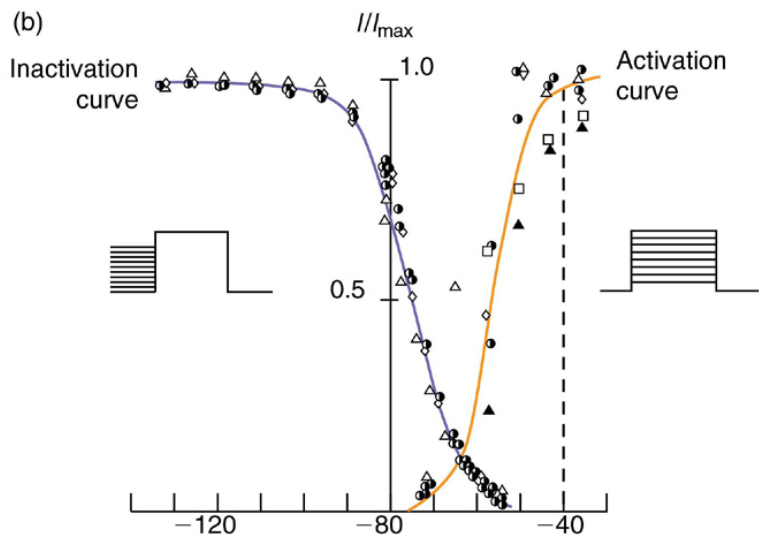
\includegraphics[width=0.5\linewidth]{Pictures//Anakin/activ-inactiv.png}
    \caption{Activation (right curve) and inactivation (left curve) curves obtained from nine different experiments. The voltage protocols used are shown in insets. In the ordinates, I/Imax represents the ratio of the peak \gls{Na} current (I) recorded at the tested \gls{gls:Pote} of the abscissae and the maximal peak \gls{Na} current (Imax) recorded in this experiment. (From Chiu Sy, ritchie JM, bogart rb, Stagg d (1979) A quantitative description of \gls{gls:membrane} currents from a rabbit myelinated nerve. J. Physiol.292, 149–166) }
    \label{fig:enter-label}
\end{figure}

\subsection{The repolarization phase of the sodium-dependent action potential results from sodium channel inactivation and partly from potassium channel activation}
%\subsection{The \gls{gls:repol} phase of the \gls{Na}-dependent \gls{ap} results from  \gls{Na} channel inactivation and partly from \gls{K} channel activation}

The voltage-gated Ka+ channel type that participates in \gls{gls:membrane} \gls{gls:repol} are the so called delayed rectifiers, which activate after a delay following \gls{gls:membrane} \gls{gls:depol} and inactivate slowly. The function of the delayed rectifier channel is to transduce, with a delay, \gls{gls:membrane} \gls{gls:depol} into an exit of K+ \glspl{gls:ion}. 

The gating behavior of the delayed rectifier channel is different from that of the Na+ channel.  Whereas all four voltage-sensitive domains in K+ channels must be activated in order for pore opening to occur, Na+ channel pore opening requires activation of only three voltage-sensitive domains. Thus, part of the difference in activation speed between Na+ and K+ channels may be due to the lesser number of voltage-sensitive domains required to move in Na+ channels.

The average open time \(\tau_O\) measured in the patch illustrated in Figure10 is 4.6ms. The mean closed time \(\tau_c\) is 1.5ms. As seen in the figure, during a depolarizing pulse to \qty{0}{\mV} the delayed rectifier channel spends much more time in the open state than in the closed state: at \qty{0}{\mV} its average open probability is high (po=0.76).

In order to test whether the delayed rectifier channels show some inactivation, long-lasting recordings are performed. Though no significant inactivation is apparent during test pulses in the range of seconds, during long test \glspl{gls:depol} (in the range of minutes) the channel shows steady-state inactivation at positive holding potentials (not shown). Therefore, in the range of seconds, the inactivation of the delayed rectifier channel can be omitted: the channel fluctuates between the closed and open states:
\[C\rightleftharpoons O\]
The transition from the closed (C) state to the open (o) state is triggered by \gls{gls:membrane} \gls{gls:depol} with a delay. The delayed rectifier channel activates in the range of milliseconds. In comparison, the Na+ channel activates in the range of submilliseconds. The O to C transitions of the Na+ channel frequently happen though the \gls{gls:membrane} is still depolarized. It also happens when the \gls{gls:membrane} repolarizes. 
  \begin{figure}[H]
      \centering
      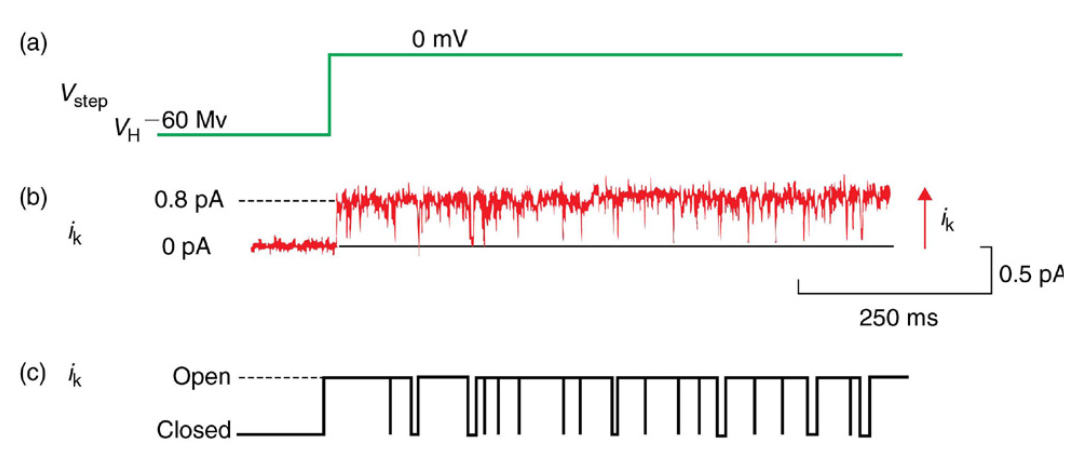
\includegraphics[width=0.5\linewidth]{Pictures//Anakin/K+channel.png}
      \caption{Single K+ channel openings in response to a depolarizing step. The activity of a single delayed rectifier channel expressed from rat brain is recorded in patch clamp (inside-out patch). A depolarizing step to \qty{0}{\mV} from a holding \gls{gls:Pote} of \qty{-60}{\mV}(a) evokes the opening of the channel (b). The elementary current is outward. The channel then closes briefly and reopens several times during the \gls{gls:depol}, as shown in the drawing (c) that interprets the current trace. bathing solution or \gls{gls:incell} solution (in mM): 100 KCl, 10 eGTA, 10 HepeS. pipette solution or \gls{gls:excell} solution (in mM): 115 NaCl, 2 KCl, 1.8 CaCl2, 10 HepeS. Adapted from Stühmer W, Stocker M, Sakmann bet al. (1988) potassium channels expressed from rat brain cdNA have delayed rectifier properties. FEBS Lett.242, 199–206, with permission. }
      \label{fig:enter-label}
  \end{figure}

The K+ channel has a constant unitary \gls{gls:contan} \(\gamma_K\). In Figure 11a, unitary currents are shown in response to increasing depolarizing steps from -50 to \qty{20}{\mV} from a holding \gls{gls:Pote} of \qty{-80}{\mV}. It can be observed that both the amplitude of the unitary current and the time spent by the channel in the open state increase with \gls{gls:depol}. 

When the mean amplitude of the unitary K+ current is plotted versus \gls{gls:membrane} test potential, a linear \(i_K/V\) relation is obtained.  This linear \(i_K/V\) relation (between -50 and \qty{20}{\mV}) is described by the equation \(i_K = \gamma_K(V-E_K)\), where V is the \gls{gls:mPote}, \(E_K\) is the reversal \gls{gls:Pote} of the K+ current, and \(\gamma_K\) is the \gls{gls:contan} of the single delayed rectifier K+ channel, or unitary \gls{gls:contan}. 

Linear back-extrapolation gives a reversal \gls{gls:Pote} value around -90/\qty{-80}{\mV}, a value close to \(E_K\) calculated from the Nernst equation. This means that from \qty{-80}{\mV} to more depolarized potentials, which correspond to the physiological conditions, the K+ current is outward. For more hyperpolarized potentials, the K+ current is inward. The value of \(\gamma_K\) is given by the slope of the linear \(i_K/V\)curve. It has a constant value at any given \gls{gls:mPote}. This value varies between 10 and 15pS depending on the preparation. 

\begin{figure}[H]
     \centering
     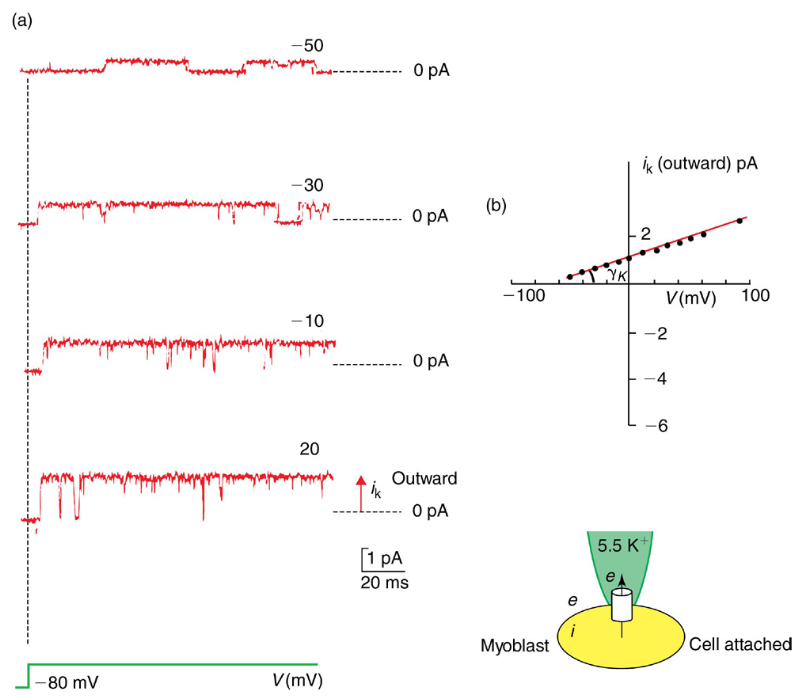
\includegraphics[width=0.5\linewidth]{Pictures//Anakin/I-V.K.png}
     \caption{The single-channel current/voltage (iK/V) relation is linear.delayed rectifier K+ channels from rat brain are expressed in a myo-blast cell line. (a) The activity of a single channel is recorded in patch clamp (cell-attached patch). unitary currents are recorded at different test potentials (from \qty{-50}{\mV} to \qty{20}{\mV}) from a holding \gls{gls:Pote} at \qty{-80}{\mV}. bottom trace is the voltage trace. (b)iK-V relation obtained by plotting the mean amplitude of iK at the different test potentials tested. iK reverses at =\qty{-75}{\mV} and gK=14pS. Intrapipette solution (in mM): 145 NaCl, 5.5 KCl, 2 CaCl2, 2 MgCl2, 10 HepeS. Adapted from Koren G, liman er, logothetis deet al. (1990) Gating mechanism of a cloned potassium channel expressed in frog oocytes and mammalian cells. Neuron2, 39–51.}
     \label{fig:enter-label}
 \end{figure} 

The macroscopic delayed rectifier K+current (IK) has a delayed voltage dependence of activation and inactivates within tens of seconds. Whole cell currents start to activate at potentials positive to \qty{-30}{\mV} and their amplitude is clearly voltage dependent. When unitary currents recorded from 70 successive depolarizing steps to \qty{0}{\mV} are averaged (Figure4.20b), the macroscopic outward current obtained has a slow time to peak (4ms) and lasts the entire depolarizing step. The whole cell current amplitude at steady state (once it has reached its maximal amplitude) for a given \gls{gls:Pote} is
\[I_K= N p_o i_K,\]
where N is the number of delayed rectifier channels in the \gls{gls:membrane} recorded, \(p_o\) the open probability at steady state and iK the elementary current. The number of open channels Npo increases with \gls{gls:depol} (to a maximal value) and so does IK. 

The IK/V relation shows that the whole cell current varies linearly with voltage from a threshold \gls{gls:Pote} which, for those conditions, is around \qty{-40}{\mV} . When the \gls{gls:membrane} is more hyperpolarized than the \gls{gls:tPote}, very few channels are open and IK is equal to zero. For \glspl{gls:mPote} more depolarized than the \gls{gls:tPote}, IK depends on \(p_o\) and the driving force state (V-EK) which augments with \gls{gls:depol}. once \(p_o\) is maximal, IK augments linearly with \gls{gls:depol} since it depends only on the driving force. 
\begin{figure}[H]
    \centering
    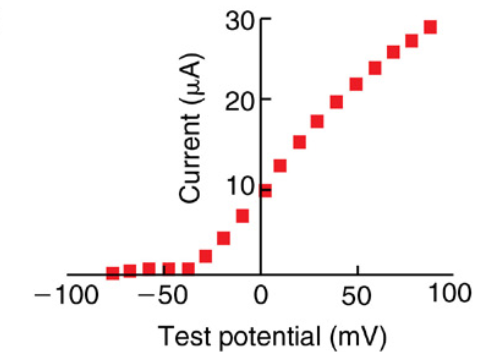
\includegraphics[width=0.5\linewidth]{Pictures//Anakin/IK-V.png}
    \caption{Characteristics of the macroscopic delayed recti-fier K+ current.  The amplitude of the current at steady state is plotted against test potential. The \gls{gls:Pote} threshold for its activation is \qty{-40}{\mV}.  }
    \label{fig:enter-label}
\end{figure}
In conclusion, owing to their delay of opening, delayed rectifier channels open when the \gls{gls:membrane} is already depolarized by the entry of Na+ \glspl{gls:ion} through open voltage-gated Na+ channels. Therefore, the exit of K+ \glspl{gls:ion} does not occur at the same time as the entry of Na+ \glspl{gls:ion}. This allows the \gls{gls:membrane} to first depolarize in response to the entry of Na+ \glspl{gls:ion} and then to repolarize as a consequence of the exit of K+ \glspl{gls:ion}.
 \begin{figure}[H]
     \centering
     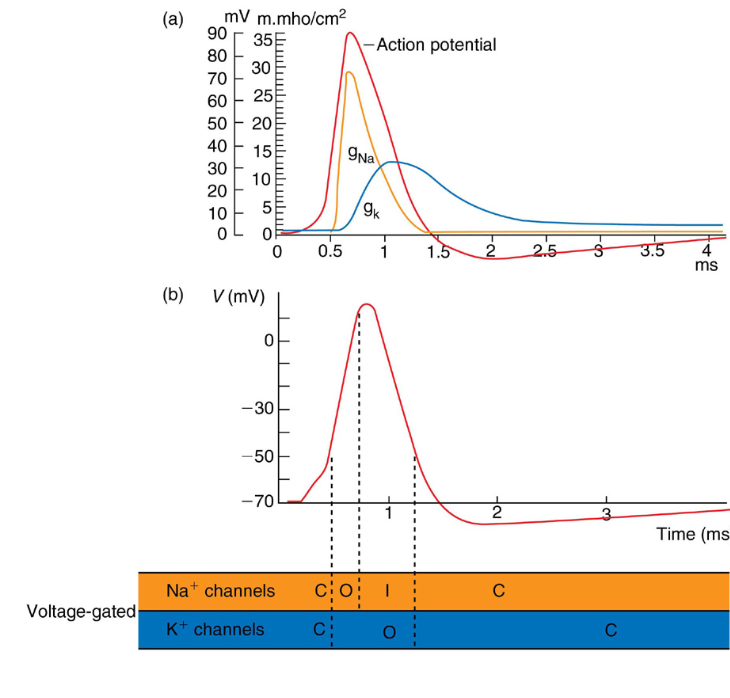
\includegraphics[width=0.5\linewidth]{Pictures//Anakin/N.K.png}
     \caption{Gating of Na+ and K+ chan-nels during the Na+-dependent action potential.(a) Interpretation of the manner in which the con-ductances to Na+ and K+ contribute to the action potential. (b) State of the Na+ and K+ voltage-gated channels during the course of the action potential. o, channels open; I, channels inactivate; C, channels close or are closed. Trace (a) adapted from Hodgkin Al, Huxley AF (1952) A quantitative description of \gls{gls:membrane} current and its application to conduction and excitation in nerve. J. Physiol.117, 500–544.}
     \label{fig:enter-label}
 \end{figure}
 \end{document}